\subsection{Main Problem}
\begin{itemize}
	\item The aim of this simulation is observe the movement of wettable fluid (blue) from the region of thicker tube to the thinner tube.
	\item The saturation of each phase is measured in the region of thinner tubes.
	\item All boundaries are closed, the saturation of a phase for the whole system remains constant in time.
	\item The radius in the outer region is three times larger.
\end{itemize}



\subsection{Result for Imbibition 10x10}
	\subsubsection{Figures}
		\begin{figure}[H]
			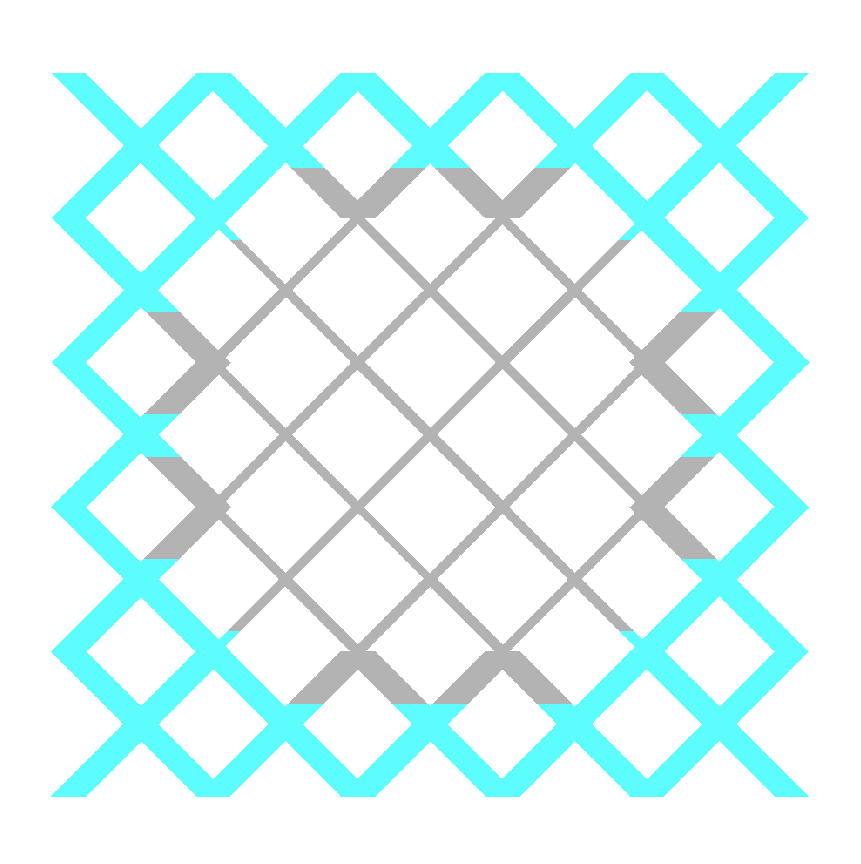
\includegraphics[height=8cm]{fig_result10by10_1}
			\caption{Initial setup, outer radius is 3 times larger than inner.}
			\label{fig_invasion-result1}
		\end{figure}
		
		\begin{figure}[H]
			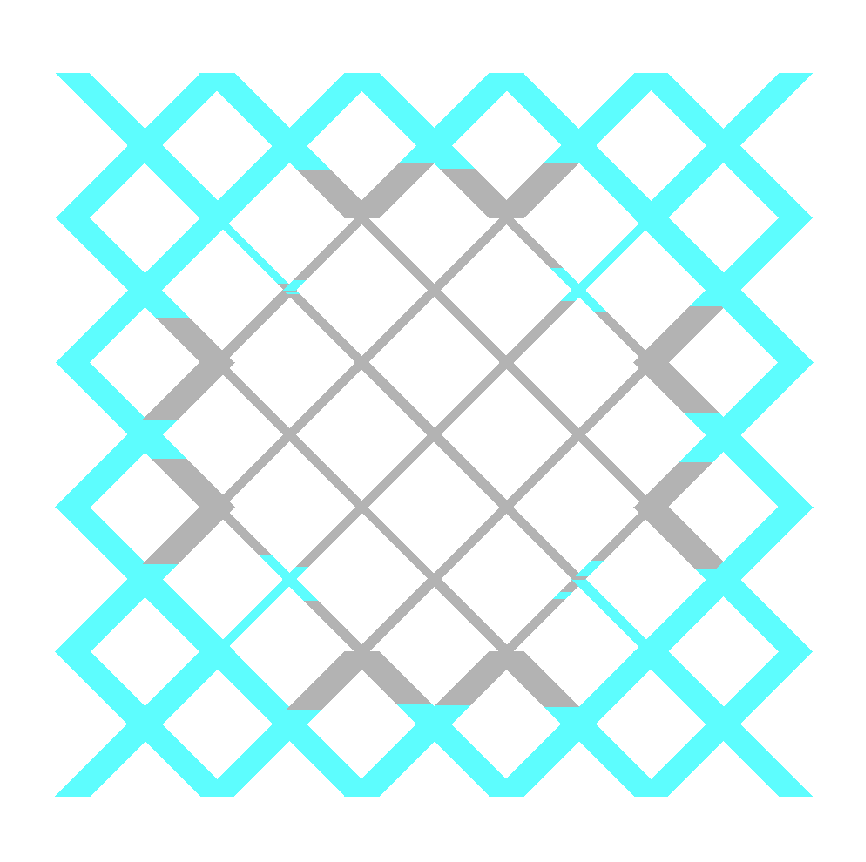
\includegraphics[height=8cm]{fig_result10by10_2}
			\caption{Showing invasion of wetting(blue) fluid into the region which contains thinner radius. The flow accelerates because, for a corner initially there are 3 meniscus, it multiplies into 3 when the meniscus reaches the node. The corner where the meniscus reaches the node late is pushed back because of the excessive pressures from the other corners.}
			\label{fig_invasion-result2}
		\end{figure}
		
		
		\begin{figure}[H]
			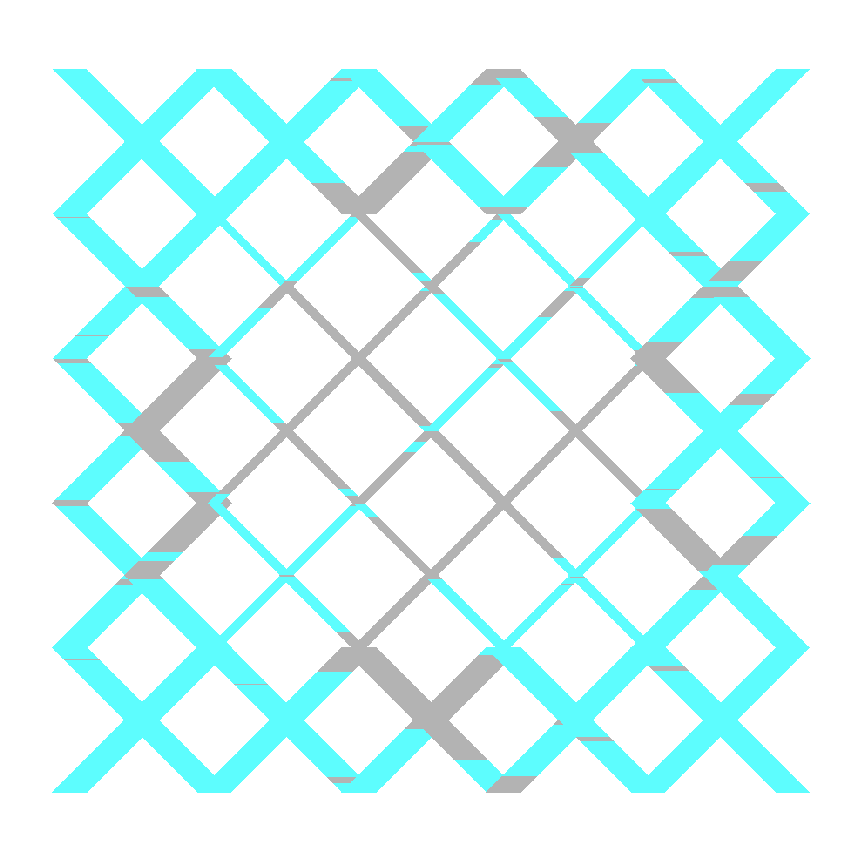
\includegraphics[height=8cm]{fig_result10by10_3}
			\caption{The invasion slows down and possibly oscillates, it is due to the meniscus in the inner region being ineffective to suck more blue fluid as most tubes have two meniscus. In our algorithm, tubes with two meniscus have a zero net pressure.}
			\label{fig_invasion-result3}
		\end{figure}
	
	\subsubsection{Plot}
		\begin{figure}[H]
			\centering
			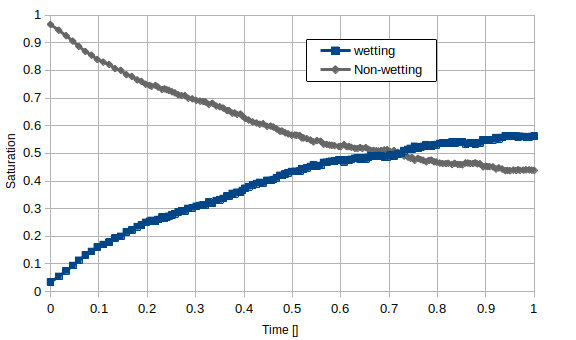
\includegraphics[width=0.8\textwidth]{fig_plot-sat-vs-time}
			\caption{Plot of saturation of blue fluid in the region of thinner radius with respect to time, here the time is without dimensions.}
			\label{fig_plot-sat-vs-time}
		\end{figure}
		
		For the simulations the length of each tube was taken to be unity and only the ratio of viscosity was used in equation \ref{eq:flow-rate-main}, since these values do not change the geometry of the flow and change only the scale of time. Dimensionless value of time was used.
		
	\subsubsection{Discussion}
		\begin{enumerate}
			\item The blue fluid has approximately logarithmic dependence with time, the invasion rapidly rises and slows down, until it becomes almost constant. The calculation was stopped after 150 steps, because there was very small progress after it. Note that the time step for each step is different.
			\item The blue fluid enters up to $0.56$ of the saturation.
			\item The saturation vs time appears similar to the ones in the reference \cite{aker1998two}, \cite{fatt1956network}.
		\end{enumerate}

		
\subsection{Result for Imbibition 26x26}
	
	\subsubsection{Figures}
		\begin{figure}[H]
			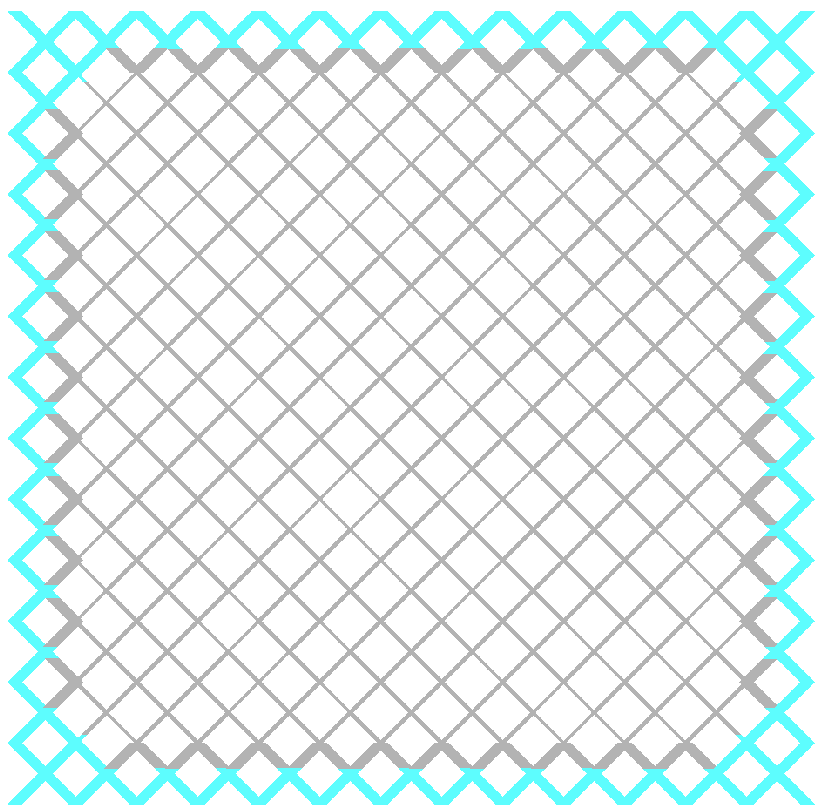
\includegraphics[height=8cm]{fig_result26by26_1}
			\caption{Initial setup}
		\end{figure}
		
		\begin{figure}[H]
			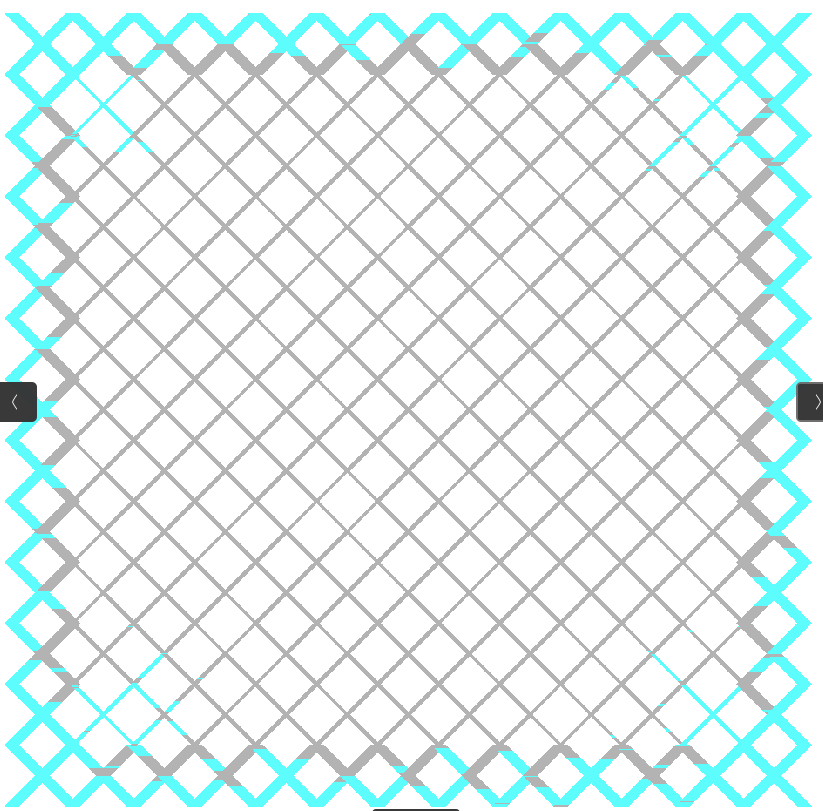
\includegraphics[height=8cm]{fig_result26by26_2}
			\caption{Acceleration}
		\end{figure}
		
		
		\begin{figure}[H]
			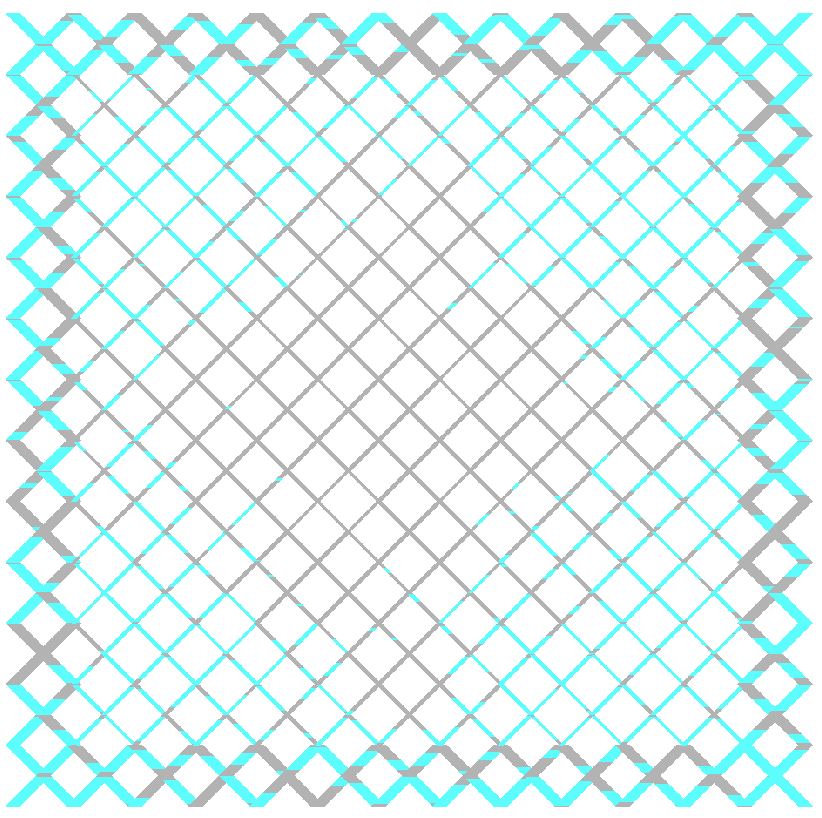
\includegraphics[height=8cm]{fig_result26by26_3}
			\caption{Slowing down}
		\end{figure}
		
		\begin{figure}[H]
			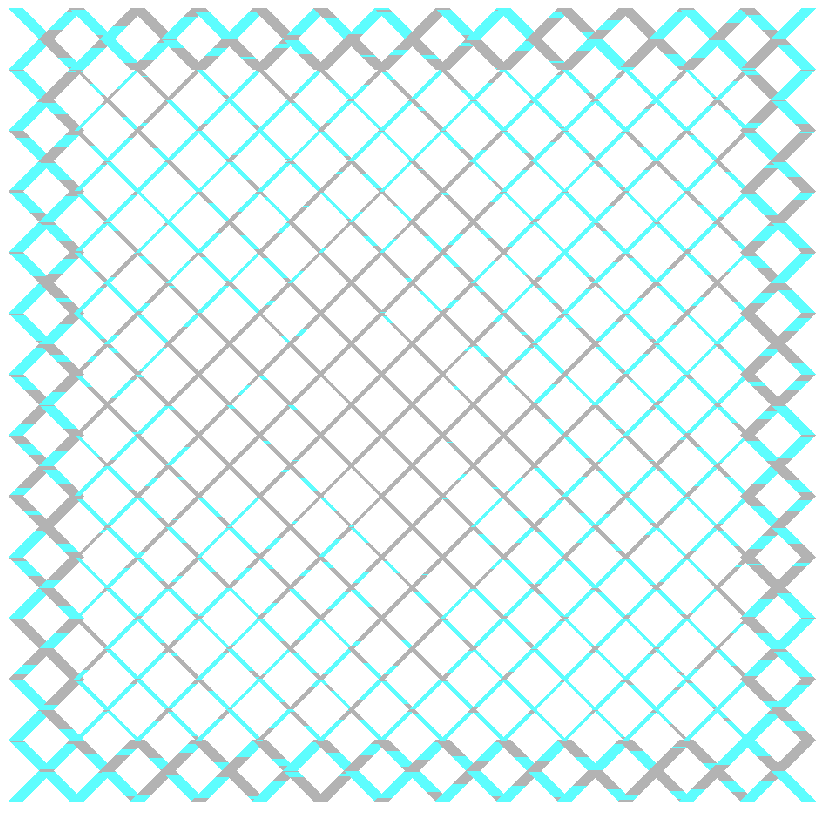
\includegraphics[height=8cm]{fig_result26by26_4}
			\caption{Final}
		\end{figure}
	
	\subsubsection{Plot}
		\begin{figure}[H]
			\centering
			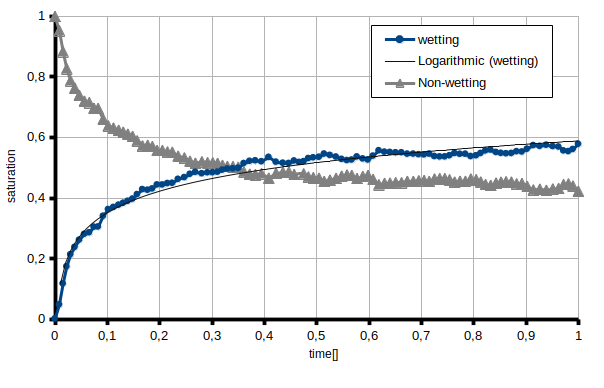
\includegraphics[width=0.8\textwidth]{fig_plot-sat-vs-time2}
			\caption{Plot of saturation of blue fluid in the region of thinner radius with respect to dimensionless time.}
		\end{figure}
		
	\subsubsection{Discussion}
		\begin{enumerate}
			\item Calculation was done for 20,000 steps.
			\item Plot for every 200 frames.
			\item Equal volumes of each phases.
			\item The saturation for wetting fluid is $0.57$ for the inner region, which is very close the previous simulation for 10x10. 
			\item It is clear that the relaxation parameter is present as the saturation converges to an equilibrium value.
		\end{enumerate}
	
